\chapter{Backgroud}

As the proposed architecture and algorithm extend existing work on Probablistic Graphical Models, a substantial amount of background is required culminating with the new approach being derived. An robust understanding of these concepts is required for this project to implement and design appropriate evaluations for the proposed architecture new approach.

\section{Generative Models}\label{S:Generative-Models}

This project works with nueral network based generative models.
Generative models are a powerful way to model data. The rational behind them being that we aim to learn a model that can both create the training data represent it, and reconstruct it using it's learned representation. Generative models can map input data from raw values to higher level features. Hinton~\cite{hinton:32723:vv} gave a compelling argument for higher level features in the context of generative models. \begin{quote} Consider, for example, a set of images of a dog. Latent variables such as the position, size, shape and color of the dog are a good way of explaining the complicated, higher-order correlations between the individual pixel intensities, and some of these latent variables are very good predictors of the class label.\end{quote}

Generative models model a distribution over a collection binary variables $X$, where $X$ is comprised of variables which can be observed or unobserved. The observed variables are referred to as \texttt{visible} variables or units ($v$). Conversely, unobserved variables correspond to the hidden units of the neural network ($h$). With these terms defined the joint distribution that generative models model can be expressed as $P(X)$ where $X$ is comprised of $h,v$. Collections of these units, are often referred to as `patterns` or `vectors` in that they are represented by a vector or pattern of bits. For instance in the context of an image, a visible pattern is the pixels of the image flattened into a one dimensional vector.

\section{Directed PGMs}

The new approach proposed in this project uses both the two classes of Probablisitic Graphical Models, Directed and Undirected. A Directed PGM, is a notation for factorising over a collection of stochastic variables.
Given $X$, the variables in the generative model, and $parent_i$ the parent unit of $x_i$, the distribution over $X$ in a directed PGM is defined by the following factorisation:
\begin{equation}\label{eq:sbn-factorisation}
P(X) = \prod_i P(x_i | parent_i)
\end{equation}
Connections between units in the Directed PGM express causation~\cite{pearl2014probabilistic}. They provide an expressive way to represent a collection of related, stochastic variables. See figure \ref{F:PGM-example} for the minimal example, where variable $A$ is dependent on $B$. As a result this network often referred to as a Belief Network or Bayesian Network where it's causal dependencies are expressed as a conditional probability table or `factor`. For example in figure \ref{F:PGM-example} the probabilities of $A$ being in a given state are dependent on $B$. The joint distrubution over $A$ and $B$, as in equation \ref{eq:sbn-factorisation}, can be expressed as:
$$P(A,B) = P(A|B)P(B)$$
\begin{wrapfigure}{r}{0.2\textwidth}
\begin{center}
  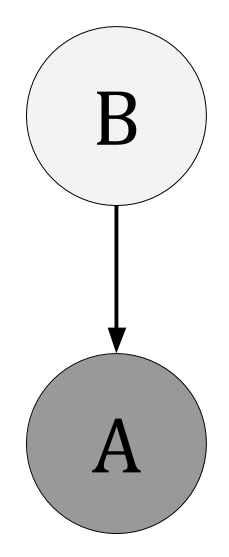
\includegraphics[width = 0.1\textwidth]{Assets/PGM_Example_1.png}
\caption{Minimal Directed PGM, showing an observed variable `A` and it's hidden cause `B`.}
\label{F:PGM-example}
\end{center}
\end{wrapfigure}

\todowording{consider removing ---
Note that a normalisation is not needed in DPGMs as the conditional probabilities enforce that the factors sum to 1.}

\subsection{Explaining Away in DPGMs}

\todowording{A common task in generative models is given a known parent unit (a cause), is inferring the probability of children variable dependent on that parent being in a given state. In directed PGMs this proves trivial to calculate. The opposite task of inferring the state of causes, given the effect of that cause is also a desirable task\todocite{}. It becomes problematic in DPGMs as these causal relationships gives rise to the effect of `Explaining Away`. The canonical example \texttt{Burglar, Earthquake, Alarm Problem} is a exemplifies this effect effect\cite{Barber:2012:BRM:2207809} and is illustrated in figure \ref{F:Explaining-Away}.}
\begin{figure}[h]
\begin{center}
  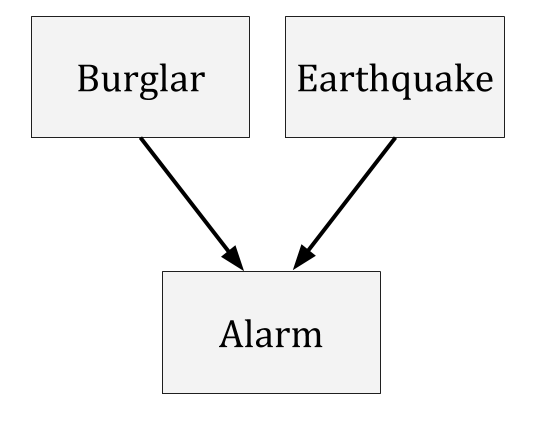
\includegraphics[width = 0.4\textwidth]{Assets/Explaining_Away.png}
\caption{The famous Burglar, Earthquake, Alarm network showing a minimal case of explaining away.}
\label{F:Explaining-Away}
\end{center}
\end{figure}
Knowledge of the state of the \texttt{alarm} makes \texttt{burglar} and \texttt{earthquake} dependent. The \texttt{alarm} is the observable variable here ($v$) and the \texttt{burglar} and \texttt{earthquake} are the hidden `causes` ($h$). For example if the \texttt{alarm} is true, and we see news of earthquake in the area, our belief that we have been burgled decreases. Expressed (again exemplify equation \ref{eq:sbn-factorisation}) in probabilities where $A$, $B$ and $E$ are the states of \texttt{alarm},\texttt{burglar} and \texttt{earthquake} respectively:
$$
P(A,B,E) = P(A|B,E)P(B)P(E)
$$

\subsection{Directed PGMs in Neural Networks: The Sigmoid Belief Network}

A Belief network can be expressed as a neural network, where conditional probabilities are parameterised as weights. \todowording{Simplify --- This network is called a Sigmoid Belief Network (SBN) as the probability of a variable $x_i$ being 1 that is dependent on a ancestor variable $parent_i$ the weighted sum into $x_i$, $\phi_i$ passed through the sigmoid function ($ \sigma(x)=1/(1+e^{-x})$)}. This is equivalent to a perceptron using a sigmoid activation function and ensures that the output is a valid probability (between 0 and 1).
SBNs take a naive approach to causes, where each hidden unit represent a single, simple cause. Formally, $\phi_i$ is a weighted sum of the activations of parent nodes:
$$ \phi_i = \sum_{j \in parent_i} W_{ij}x_j$$
and
$$
P(x_i = 1 | parent_i) = \sigma(\phi_i)
$$

\section{Undirected PGMs:}

Undirected PGMs do not represent causation, instead merely capturing a dependency between two units. These pairwise dependencies change the structure of the factorisation a factor $\Phi$ between each pair of variables $x_i,x_j$ resulting in the factorisation:
$$
P(X) = \frac{1}{Z} \prod_i \Phi(x_i, x_j)
$$
The introduction of the normalisation $Z$ (often referred to as the partition function) adds nontrival complexity to performing inference in Undirected PGMs~\todocite{}, a sum over all $2^N$ configuratiions of $x$ is required.

On the other hand, Undirected PGMs do not capture causal relationships. Calculating the state of a variable given another is no longer hampered by the effect of explaining away, however their reccurent structure, while expressive introduces an intractability in practice.

\subsection{Undirected PGMs in Neural Networks: The Boltzmann Machine}
A UPGM expressed as nueral network is referred as Boltzmann Machine or Markov Field, where connections encode dependancies with an associated weight. We see this where $W_{ij}$ is the weight between variables $x_i$ and $x_j$ the factor $\Phi$ is expressed as:
$$
\Phi(x_i, x_j) = e^{x_ix_jW_{ij}}
$$
The Boltzmann machine has proposed in various forms, from different domains throughout the years, for instance it was presented in a non-stochastic context of the Hopfield network in~\cite{Hopfield01041982}. Hinton and Sejnowski also proposed the Boltzmann machine in~\cite{geoffreye.hintonterrencej.sejnowski1983}. An example Boltzmann Machine is shown in figure \ref{F:Boltzmann-Machine}. As shown in this figure \ref{F:Boltzmann-Machine}, the Boltzmann Machine can be recurrent, expressing complex dependencies between variables. This recurrence makes inferring the state of a subset variables based on knowledge of another subset non-trivial as the size of the network grows\todocite{}.
\begin{figure}[h]
\begin{center}
  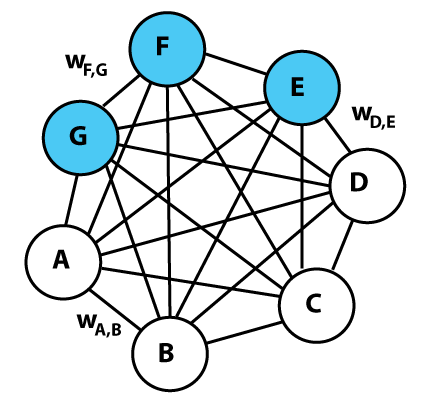
\includegraphics[width = 0.4\textwidth]{Assets/Boltzmann_Machine.png}
\caption{A Boltzmann Machine, the blue shaded nodes representing the observed variables, and the non-shaded nodes the latent variables.}
\label{F:Boltzmann-Machine}
\end{center}
\end{figure}

\subsection{Restricted Boltzmann Machines}


\todowording{A Boltzmann Machine's architecture can be altered to alleviate inference shortcoming. The restriction, originally proposed by \cite{Smolensky:1986vy}, and then later revitalised with a training algorithm that operates on the deeper architecture of the DBN~\cite{geoffreye.hintonterrencej.sejnowski1983}}. The restriction requires the network to be a two layer bipartite network, each layer corresponding to the observed (visible) and latent (hidden) units. Connections are forbidden between the layer of hidden units and the layer of visible units respectively. An example Restricted Boltzmann Machine architecture is shown in figure~\ref{F:Restricted-Boltzmann-Machine}. The collection of hidden units, forming a layer are referred to as the \texttt{hidden layer}. The collection of visible units are referred to as the \texttt{visible layer}.

\begin{figure}[h]
\begin{center}
  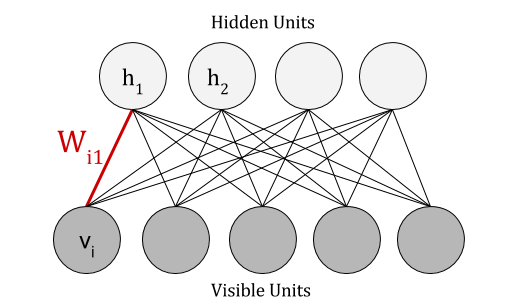
\includegraphics[width = 0.6\textwidth]{Assets/RBM_Example.png}
\caption{An example Restricted Boltzmann Machine with four hidden units, and five visible units. Note that the edges between units are not directed - representing a dependency not a cause. }
\label{F:Restricted-Boltzmann-Machine}
\end{center}
\end{figure}

% \subsection{Energy, and the log likelihood of the joint}
%
% An RBM models the joint distribution of hidden and visible states.
% The RBM assigns to every configuration of $h$ and $v$ an \texttt{Energy}, where the lower the energy, the more likely the RBMs configuration is to \textit{fall} into that state. Hopfield, in the context of what is now called the Boltzmann Machine~\cite{Hopfield01041982}, presented this energy as defined by the function as:
% $$ E(v,h) = -\sum_{i \in visible}{W_{0i}v_i}   -\sum_{j \in hidden}{W_{0j}h_j}  -\sum_{i,j}{v_ih_jW_{ji}}  $$
The probability of the RBM being in a given configuration is the joint probability of $h$ and $v$:
$$ P(h,v) = \frac{1}{Z} \prod_{j,i} e^{h_jv_iW_{ji}} $$
Taking logs this becomes:
$$ \log P(h,v) = \log \sum_{j,i} h_jv_i  W_{ji}  - \log Z $$
$ Z $ is the partition function, which normalises the probability of the joint. Calculating this would require summing over all $2^N$ configurations of $h$ and $v$, which is intractable for practical numbers of units. For instance a 28 by 28 image corresponds to 784 visible units, and for, say 10 hidden units this would amount to $ 2^{784} * 2^{10} $ possible configurations. We opt to work in terms of $P^\star$ which is the non-normalised probability of the joint over $h \text{ and } v$.
% So we arrive at:

\begin{equation}\label{eq:LogPJoint}
   \log P^\star(h, v) = \log \sum_{i,j} {h_j v_i W_{ji}}
\end{equation}

\section{Sampling in Generative Models}

\subsection{Why sampling is important}

Sampling is used when the distribution we want to work from is intractable to calculate analytically. As mentioned in \ref{S:Generative-Models}, the power of generative models is their ability to represent, reconstruct and be trained on data. These tasks all require sampling from configurations of the hidden and visible units, often conditioned one or the other. There are two cases:
\begin{itemize}
  \item Sampling from $P(v|h)$, which is known as running the generative model, where the model \emph{generates} data based on a hidden representation.
  \item Sampling from $P(h|v)$, which is known as \emph{inverting} a generative model (This is also refferred to as \emph{inference}). The process is called `Inverting` because instead of the model generating the data (sampling from $P(v|h)$) we instead try to infer a representation given data $P(h|v)$. It is the process of reasoning about what we do not know, given that of which we do.
\end{itemize}


Sampling from $P(v|h)$ and $P(h|v)$ is required to train generative models, as often the gradient to be climbed/descended involves calculating a probability over all the units in the generative model. Training a network based generative model involves calculating a weight update, which in turn requires inferring a hidden representation given a training item. The converse, sampling from a $P(v|h)$ is also required. \todocite{EM}

\todowording{inference for our purpose is used for (somehting about not training)}

\subsection{The sampling technique: Gibbs Sampling}

Gibbs sampling is a special case of Markov Chain Monte Carlo \cite{hastings70}, a technique for drawing sampling from a complex distribution. Sampling from the probability mass (or `joint distribution`) of a generative model is a common use case for Gibbs sampling~\cite{Pearl:1988:PRI:52121}.

Gibbs sampling explores the desired probability distribution, taking samples of that distribution's state, allowing iterations of exploration between drawing of a sample to ensure that the samples are independent\todocite{}. The process of taking a step between states is referred to as a \texttt{Gibbs iteration} or a \texttt{Gibbs Step}. Formally the algorithm is descibed in algorithm~\ref{Alg:Gibbs-Sampling}.

\begin{algorithm}[!ht]
 \KwData{A vector $x$ indexed by $j$.}
 \KwResult{Gibbs sampling algorithm}
 Let $ x_{\smallsetminus} j$ be all components that make up $x$ vector except $x_j$\;
 initialization, begin with $x$, we are going to get a sample $x'$\;
  \For{$k$ many iterations}{
   \For{each component in $x$, $x_j$}{
     Draw a sample, $x_j'$ from $P(x_j| x_{\smallsetminus} j)$\;
     Update the current value of $x_j$ in $x$ with $x_j'$\;
   }
  }
 \caption{The Gibbs Sampling Algorithm}\label{Alg:Gibbs-Sampling}
\end{algorithm}

\subsubsection{Mixing Time of the Gibbs Sampler}

MCMC methods aim to approximate a distribution, by exploring likely states. As we often start this process from a random state, it's important that enough Gibbs steps are taken before a sample is drawn. This is because the random state may not be close any part of the true distribution we want to sample from, so by running the chain for many iterations we increase the likelihood of samples being from the desired distribution.

This process of waiting for enough steps to before drawing samples is referred to as the \texttt{Mixing Time}. When Hinton when proposed a fast training for algorithm for RBMs and DBNs~\cite{Hinton:2006:FLA:1161603.1161605}, Gibbs sampling is used for performing inference in RBMs and as result also in the ORBM. The \texttt{mixing time}, that is how many Gibbs iterations are needed to reach a satisfactory sample is an important part issue in the ORBM, in that one Gibbs step was sufficient in practice for training and using an RBM. The new generative model is not so fortunate.



\subsection{Sampling in a Sigmoid Belief Network}


Sampling from $ P(v|h) $ (known as Ancestral Sampling) is extremely efficient in a SBN, it does not need Gibbs sampling. It can be expressed as
\begin{equation}\label{eq:SBN-v-given-h}
P(v|h) = \sum_i v_i \log \sigma_i(h) + (1-v_i)log(1-\sigma_i(h))
\end{equation}
As this process is calcuated by propagating probabilites from the root hidden causes, it is known in a SBN as Ancestral Sampling.

Conversly, sampling from $P(h|v)$ in an SBN is intractable. Performing inference in a Sigmoid Belief network would allow source separation, as each hidden unit could represent a simple cause. The SBN would be shown an input, and could extract representations of the seperate causes that likely gave rise to the input. There exist algorithms for performing inference in Sigmoid Belief Networks. For instance, the Belief Propagation algorithm proposed by Judea Pearl~\cite{Pearl1982} operates on this encoding, calculating the probabilities of a given network state (i.e. the state of all the variables). As well as constraining the architecture to be Directed Acyclic Graph, Belief Propagation is intractable to use as the number of variables grow\todocite{}. As we want to work with cases with upwards of 100 visible and hidden nodes, these algorithms break down.

Despite the Sigmoid Belief Network being expressive and providing a succinct encoding of conditional probabilities, Gibbs sampling is intractable for SBNs of practical size~\cite{Jensen95blockinggibbs}. The issue being that the Gibbs chain takes too long to mix~\cite{neal1992:connectionist}, which arises from the the `explaining away effect`~\cite{Hinton:2006:FLA:1161603.1161605}. Calling back to the example in section \ref{}, instead of a single \texttt{burglar} or \texttt{earthquake} becoming dependant given the \texttt{alarm}, there is more in the realm of hundreds of burlgars and earthquakes all suddenly depedendant.

Being able to efficiently sample from $P(h|v)$ is also required for training generative models\todocite{em} making Sigmoid Belief Networks impractical for not only inference, but also training.




\subsection{Gibbs Sampling in a Boltzmann Machine}

Performing Gibbs sampling appears trivial in a Boltzmann Machine, in that to find the probability of a given unit being active a weighted input to that node is passed through a sigmoid function. However, in practice the recurrent nature of Boltzmann Machines makes sampling intractable as updating a node will change the probabilities of those connected. However, it was shown that given unlimited training time Boltzmann Machines could be trained, out performing the state of the art models of the time \todocite{This}.

Recall that $ x_{\smallsetminus} j$ be all components that make up $x$ vector except $x_j$ and that a Boltzmann Machine has symmetric weights ($ W_{ji} = W_{ij} $),
$$
P(x_j = 1, x_{\smallsetminus}j) = \frac{1}{1 + e^{-\sum_i w_{ji}x_i}}
$$
That is, Gibbs sampling in a Boltzmann Machine amounts to use the Sigmoid function of the weighted inputs.
\todocite{neal1992:connectionist}

\subsection{Gibbs Sampling in RBMs}

A big payoff for the restriction in an RBM is inverting the model becomes tractable, as the latent variables no longer become dependant given the observed variables. This is illustrated in figure~\ref{F:Restricted-Boltzmann-Machine} the hidden unit $h_1$ is not dependent on $h_2$ wether or not we know anything about the visible units. Firstly, this is the opposite of a SBN, where knowledge of the visible units makes the hidden units dependant. Secondly, by removing the recurence present in Boltzmann Machines, it reduces the expresiveness of the RBM network while making the RBM useable in practice as the Gibbs sampling process can stop after one Gibbs step\todocite{}.

In order to describe Gibbs sampling in the new architecture proposed, it must first be explained for a standard RBM --- The process of Gibbs sampling is as follows:
  \begin{itemize}
    \item One must sample from $P(h|v)$ giving a hidden state $\tilde{h'}$
    \item Using this hidden state, a visible state is then generated, $\tilde{v'}$, by sampling from $P(\tilde{v'}|\tilde{h'})$. This process of generating a hidden pattern, and subsequent visible pattern is referred to as a Gibbs step.
    \item This chain of Gibbs steps between sampling from $P(h|v)$ and $P(v|h)$ can then be repeated as desired, the longer the chain the closer the samples will be to the true joint distribution that the model has learnt. For training an RBM Hinton\todocite{CD-1Paper} showed that 1 step is often enough in practice, as one step is enough to infer a direction to adjust the weights in.
  \end{itemize}
  The process of updating the hidden, then visible layers forms what is referred to as the \texttt{Gibbs Chain} and is visualised at layer level in figure \ref{F:Gibbs_Chain}.
  \begin{figure}[h]
    \begin{center}
      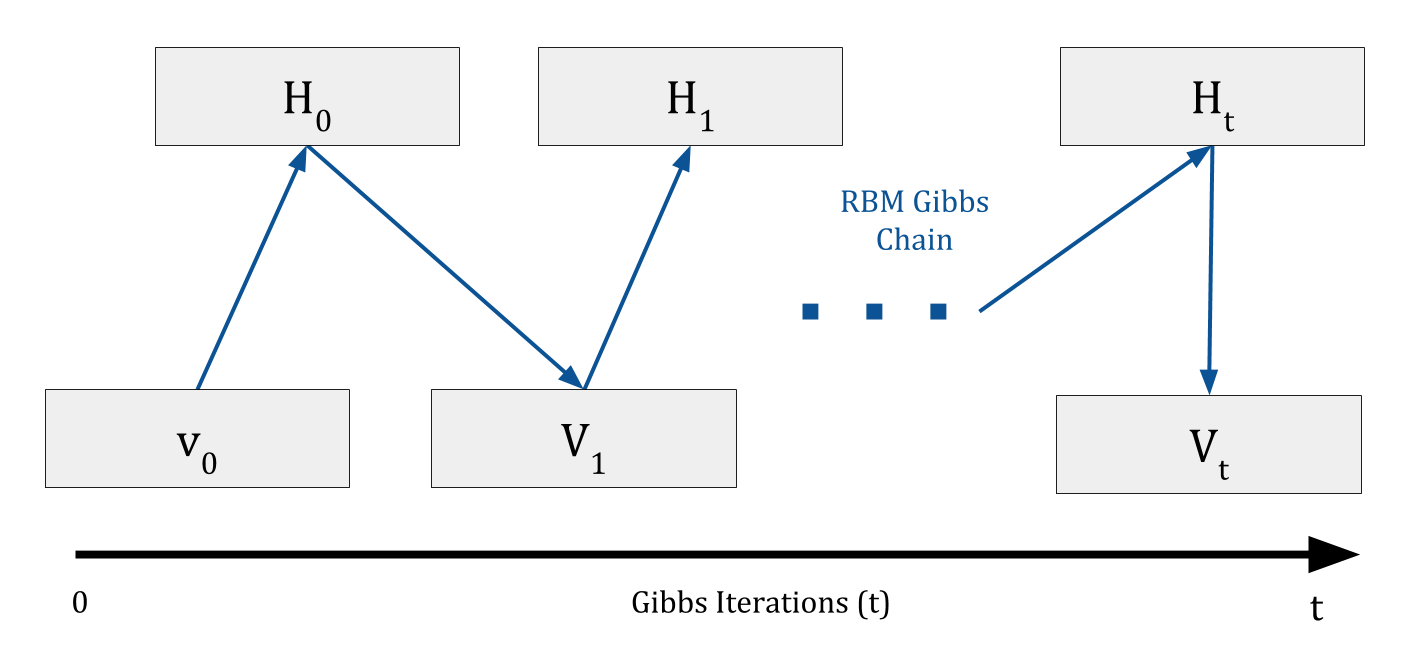
\includegraphics[width=0.8\textwidth]{Assets/RBM-Gibbs-Chain.png}
    \end{center}
    \caption{A figure illustrating a Gibbs chain where left to right indicates a Gibbs iteration. Note this is \emph{not} a PGM.}
    \label{F:Gibbs_Chain}
  \end{figure}

  \subsubsection{The Gibbs update}\label{S:Gibbs-Update}

    Denote the Gibbs sampler's probability of setting a variable, $x_j$ to 1 as:
    \begin{equation}\label{eq-p1-gibbs-full}
    P_{Gibbs}(h_j = 1 | v, h_{k != j})
    \end{equation}
    We can refer to the proability in equation \ref{eq-p1-gibbs-full} as $p_1$ and the converse $P_{Gibbs}(h_j = 0 | v, h_{k != j})$ can be referred to as $p_0$.
    Then, by the product rule of probabilities:
    $$
    \begin{aligned}
    \frac{p_1}{p_0} &= \frac{P^\star(h,v \text{ where } h_j = 1)}{P^\star(h,v \text{ where } h_j = 0)}\\
    &= \frac{p_1}{1 - p_1} \\
    % \text{Rearranging to give p_1 leads to} \\
    p_1 &= \frac{1}{1 + \frac{P^\star(h,v \text{ where } h_j = 0)}{P^\star(h,v \text{ where } h_j = 1)} }
    &= \frac{1}{1 + e^{-\psi_j}}
  \end{aligned}
    $$
  To update a hidden unit $h_j$
  we find $ P(h_j = 1 | v) $ where $v$ is an input pattern. In the context of an image, $ v $ would be the pixel values where each pixel corresponds to a visible unit, $v_i$.
  The probability of a given hidden unit activating is: \todocite{Gibbs sampling would be good here}.
    \begin{equation}\label{eq:Hid-Gibbs-Update}
    P(h_j = 1 | v) = \sigma(\psi_j)
    \end{equation}
    Where $\psi_j$ is the weighted sum into the $jth$ hidden unit and $\sigma()$ is the Sigmoid function, or it also known as the Logistic function $\sigma(x)=1/(1+e^{-x})$. Figure \ref{F:PSI} illustrates $\psi_j$ for an example RBM.
    \begin{figure}[h]
    \begin{center}
      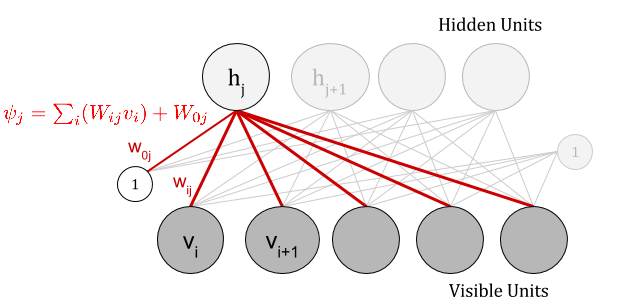
\includegraphics[width = 0.8\textwidth]{Assets/PSI_and_PHI.png}
    \caption{A diagram showing $\psi_j$, the weighted sum into the $jth$ hidden unit. Note that $W_{oj}$ is the hidden bias, represented as a unit that is always on with a weight into each hidden unit.}
    \label{F:PSI}
    \end{center}
    \end{figure}
    As the weights are symmetric, sampling from the visible layer, given a hidden state is similar. That is $P(v_i = 1 | h)$, where $h$ is the entire hidden vector is given by:
    \begin{equation}\label{eq:Vis-Gibbs-Update}
     P(v_i = 1 | h) = \sigma(\phi_{i})
    \end{equation}
    Where $\phi_i$ is the weighted sum into the $ith$ visible unit, which is: $ \phi_i = \sum(W_{ji}h_{j}) + W_{0i} $. Both $\phi_j$ and $\psi_i$ can be expressed in alternative, but useful way:
    \begin{equation}
    \phi_j = \log P^\star(v,h | v_i = 1) - \log P^\star(v,h | v_i = 0)
    \end{equation}
    \begin{equation}\label{psi-gibbs-update-rbm}
    \psi_i = \log P^\star(h,v | h_j = 1) - \log P^\star(h,v | h_j = 0)
    \end{equation}



\subsubsection{Reconstructions: visualising what the RBM has learnt}\label{SS:RBM-Reconstructions}

RBMs create an internal representation given an input by sampling from $P(h|v)$. They can also generate a faux input given an internal representation. Performing one Gibbs iteration, that is, sampling from the hidden units given a `clamped` input $ P(h|v) $ and then taking the generated hidden state and generating a faux input (sampling from $P(v|h_{sampled})$) results in a \texttt{reconstruction}. Clamped input is where the visible units are set to be an input pattern. The model tries to reconstruct the input based on the internal representation it has learnt to model. This has applications in increasing the size of a dataset by introducing variation by generatin these faux inputs\todocite{}.

\subsubsection{RBM Fanstasies: The Free-Phase of a Generative model}

In the same way that a Generative model uses reconstructions to try and recreate the supplied input vector, performing many, many (greater than 100) Gibbs iterations with no input pattern clamped allows the reconstructions to explore the probability mass that has been built by the model during training. Sampling from these wanderings creates what are refferred to as `fantasies` or `dreams`. These give a sense of what the model has learnt, and can act a smoke test for if the model has actually capture anything.
\todocite{(TODO-CITE-PAPER-WITH-MNIST-DREAM-EVALUATION, they were crappy)}.

%
% \subsection{Terminology in Generative Models observable and hidden variables}
%
% Connections between units are used to encode relationships between the variables, where the relationship may be causal, such as in a Sigmoid Belief network or an encoding/representation in the Restricted Boltzmann Machine.
%

% \subsection{PGMs as a tool reasoning about generative models}
%
% Probalistic Graphical Models or PGMs for short, are an expressive way to represent a collection of related, stochastic variables. If the graph is directed then the edges represent causation, this is also referred to a Bayesian network. Conversely, if the graph was undirected then edges represent a dependancy or mapping.

%   \section{An intractable model for causes}
%     \subsection{Sigmoid Belief Networks}
%
%     The ORBM relies on the Sigmoid Belief Network to capture the causation. The Sigmoid Belief Network (SBN) is composed of units with weights and a sigmoid activation function, akin to that of a perceptron linear threshold unit/Perceptron. The probability of a node being `on` is found by taking the weighted sum of all input to that node and applying a Sigmoid function or another activation function that ensures a values between $0$ and $1$.
%
%     SBNs offer a way to model causation in machine learning, as every hidden unit represent a single, simple cause. Nodes in the network represent binary variables which are dependent on ancestor nodes, the degree of which is encoded in a weight on a directed edge between them.
%
%
%
%     \subsection{Explaining Away --- a trade off between modeling causes and tractability}\label{SS:Explaining-Away}
%
%     The benefit of the Belief Network is also it's weakness, a structure that models a system of interest inherently has dependancies. In its minimal case explaining away can be seen in a 3 node network popularised by David Barber in his book \cite{Barber:2012:BRM:2207809}, as shown in figure \ref{F:Explaining-Away}. Each of the nodes represents a binary state. For instance $Burglar = 1$ means that the person owning the \texttt{Alarm} has been burgled. Also note how the connections between the units have arrows, this conveys causation.
%
%
%     In the network shown in figure \ref{F:Explaining-Away}, knowledge of the \texttt{Alarm} creates a dependance between \texttt{Burglar} and \texttt{Earthqaukes}. For instance, say the Alarm has gone off and we know an earthquake has occurred, our belief in being burgled decreases. The dependance in belief networks means that sampling from the network requires a longer Markov Chain to mix, as changing the value of \texttt{Earthquake}, effects the value of \texttt{Burglar}. In a network with many connected nodes the dependence introduced makes sampling take longer. In the context of images, where there may be upwards of 1000 observable values, all with different dependancies this becomes intractable. Neal showed this by comparing the number of gibbs iterations required for small enough error rates in~\cite{neal1992:connectionist}.
%
%   \subsection{Boltzmann Machines}
%
% A Boltzmann machine has proposed in various forms throughout the years from different backgrounds, for instance Paul Smolensky presented it in context of  `Harmony Theory` \cite{Smolensky:1986vy}. Where-as Hinton and Sejnowski also propsed the Boltzmann machine in~\cite{geoffreye.hintonterrencej.sejnowski1983}. The Boltzmann Machine has qualities in common with Belief Networks. Both are generative models with their nodes having probabilities of being active based on neighboring nodes. Connections between nodes have associated weights as shown in figure \ref{F:Boltzmann-Machine}. These weights are symmetric.
% Unlike a Belief Network, a Boltzmann Machine is a undirected network that allows cycles and thus more complex relationships can be captured. Also connections no longer encoe causal information, instead they encode a dependency.
%
%
%   \section{Restricted Boltzmann Machines: A Strong assumption}
%
%   While Boltzmann Machines are impractical to train and sample from as networks grow in size \todocite{} their architecture can be altered to alieviate these shortcomings. The restriction, originally proposed by \todocite{Hinton, a proper cite}, and then later revitalised with a deeper architecture training algorithm in Hintons \cite{geoffreye.hintonterrencej.sejnowski1983}. The restriction requires the network to be a two layer bipartite network, each layer corresponding to the observed (visible) and latent (hidden) units. Connections are forbidden between the layer of hidden units and the layer of visible units respectively. An example Restricted Boltzmann Machine architecture is shown in figure~\ref{F:Restricted-Boltzmann-Machine}. The collection of hidden units, forming a layer are referred to as the \texttt{hidden layer}. The collection of visible units are referred to as the \texttt{visible layer}.
%

%   \subsection{Gibbs Sampling in RBMs}
%
%   In order to describe Gibbs sampling in the ORBM, it must be first introduced in the context of RBMs. For the following discussion, the hidden units are indexed by $j$ and the visible units are indexed by $i$.
%   To perform inference, create reconstructions, and train RBMs, Gibbs sampling is used to draw samples from $P(h|v)$ (referred to as sampling from the posterior) and $P(v|h)$ respectively. It is introduced here to be reference later in Gibbs in an ORBM. In an RBM the process of Gibbs sampling is as follows:
%   \begin{itemize}
%     \item One must sample from $P(h|v)$ giving a hidden state $\tilde{h'}$
%     \item Using this hidden state, a visible state is then generated, $\tilde{v'}$, by sampling from $P(\tilde{v'}|\tilde{h'})$. This process of generating a hidden pattern, and subsequent visible pattern is referred to as a Gibbs step.
%     \item This chain of Gibbs steps between sampling from $P(h|v)$ and $P(v|h)$ can then be repeated as desired, the longer the chain the closer the samples will be to the true joint distribution that the model has learnt. For training an RBM Hinton showed that 1 step is often enough in practice, as one step is enough to infer a direction to adjust the weights in.
%   \end{itemize}
%    This process can be calculated in one step for all units in the target layer as they are independant of one another. The process of updating the hidden, then visible layers forms what is referred to as the \texttt{Gibbs Chain}. \todocite{Feel like I could  cite this again in like a CD paper or something.} This process is visualised at a layer level in figure \ref{F:Gibbs_Chain}
%
%   \begin{figure}[h]
%     \begin{center}
%       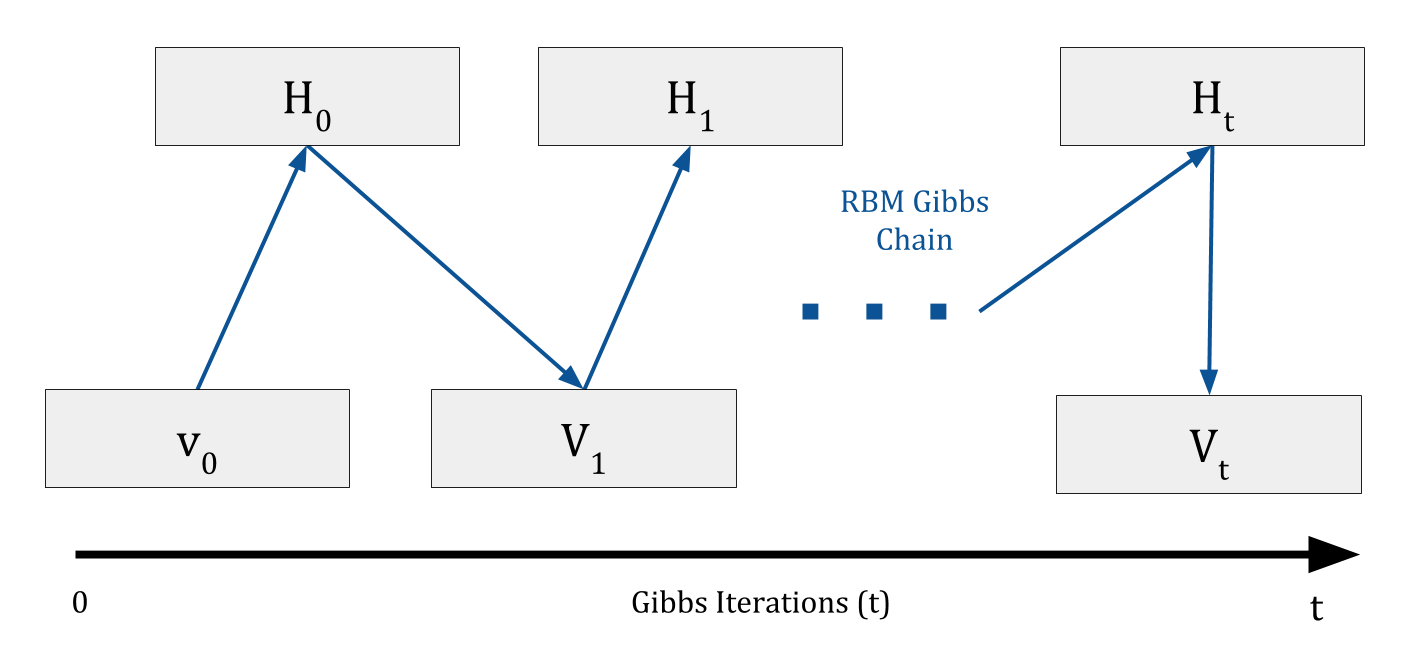
\includegraphics[width=0.8\textwidth]{Assets/RBM-Gibbs-Chain.png}
%     \end{center}
%     \caption{A figure illustrating a Gibbs chain where left to right indicates a Gibbs iteration. Note this is \emph{not} a PGM.}
%     \label{F:Gibbs_Chain}
%   \end{figure}
%
%   \subsubsection{The Gibbs update}\label{S:Gibbs-Update}
%
%   In a standard RBM, updating a hidden unit $h_j$ when performing Gibbs sampling is calculated by finding $ P(h_j = 1 | v) $ where $v$ is an input pattern. In the context of an image, $ v $ would be the pixel values where each pixel corresponds to a visible unit, $v_i$.
%   The probability of a given hidden unit activating is: \todocite{Gibbs sampling would be good here}.
%   \begin{equation}\label{eq:Hid-Gibbs-Update}
%   P(h_j = 1 | v) = \sigma(\psi_j)
%   \end{equation}
%   Where $\psi_j$ is the weighted sum into the $jth$ hidden unit and $\sigma()$ is the Sigmoid function, or it also known as the Logistic function $\sigma(x)=1/(1+e^{-x})$. Figure \ref{F:PSI} illustrates $\psi_j$ for an example RBM.
%
%   \begin{figure}[h]
%   \begin{center}
%     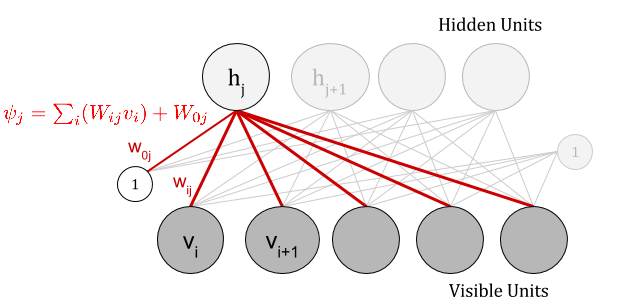
\includegraphics[width = 0.8\textwidth]{Assets/PSI_and_PHI.png}
%   \caption{A diagram showing $\psi_j$, the weighted sum into the $jth$ hidden unit. Note that $W_{oj}$ is the hidden bias, represented as a unit that is always on with a weight into each hidden unit.}
%   \label{F:PSI}
%   \end{center}
%   \end{figure}
%
%
%
%   As the weights are symmetric, sampling from the visible layer, given a hidden state is similar. That is $P(v_i = 1 | h)$, where $h$ is the entire hidden vector is given by:
%   \begin{equation}\label{eq:Vis-Gibbs-Update}
%    P(v_i = 1 | h) = \sigma(\phi_{i})
%   \end{equation}
%   Where $\phi_i$ is the weighted sum into the $ith$ visible unit, which is: $ \phi_i = \sum(W_{ji}h_{j}) + W_{0i} $. Both $\phi_j$ and $\psi_i$ can be expressed in alternative, but useful way:
%   \begin{equation}
%   \phi_j = \log P^\star(v,h | v_i = 1) - \log P^\star(v,h | v_i = 0)
%   \end{equation}
%   \begin{equation}\label{psi-gibbs-update-rbm}
%   \psi_i = \log P^\star(h,v | h_j = 1) - \log P^\star(h,v | h_j = 0)
%   \end{equation}
%
%
%
%
%     % \subsubsection{Tractable Training - Contrastive Divergence}
%     % Hinton TODO-CITE-CLASSIC-PAPER proposed Contrastive Divergence as a method for training RBMs efficiently. The algorithm leverages the now tractable wake phase because $P(h|v)$ is efficeint to compute. However the free or sleep phase required another restriction where the network is only left to its own dynamics can be limited to only one iteration and still perform well. TODO-CITE-CD-PAPER
%
%     % This restriction allows an efficient calculation of the Wake Phase of generative model learning, as the $ P(h|v) $ can be calculated as a simple weighted sum passed through a sigmoid followed by a bernouli trial where the probability of being $1$ is equal to the result of sigmoid.
%
%
%
%   % \subsection{Deep Learning}
%   %
%   %   \begin{itemize}
%   %     \item Discuss deep learning as there are clear parallels to Deep Belief Networks and the new approach
%   %     \item in paritcular how the deep networks have this process of freezing the weights and creating a sigmoid belief layer instead. There seem to be clear parallels between a deep network with one RBM to the ORBM.
%   %   \end{itemize}
%   %
%   % \begin{itemize}
%   %   \item Unrolling the gibbs chain and we are in effect training an infinite depth sigmoid beleif net (TODO-REFERENCE-HINTONS-PAPER-HERE)
%   % \end{itemize}
%
